\documentclass[aspectratio=169]{beamer}
\bibliography{References}
\usetheme{CambridgeUS}  % Theme can be adjusted if needed
\usepackage[utf8]{inputenc}
\usepackage{natbib}
\usepackage[T1]{fontenc}
\usepackage{graphicx}
\graphicspath{{./}{figures/}}
\usepackage{booktabs}
\usepackage{tikz}
\usetikzlibrary{arrows, positioning}

\title{Bitter Pills to Swallow:\\ The Enforcement Costs of Health Litigation}
\author{Darcio Genicolo-Martins \and Paulo Furquim de Azevedo}
\institute{Insper Institute of Education and Research}
\date{\today}

\begin{document}

\begin{frame}[plain]
  \titlepage
  \note{Welcome everyone. Today I will present our study titled ``Bitter Pills to Swallow: The Enforcement Costs of Health Litigation,'' co-authored with Paulo Furquim de Azevedo. This research examines how court-mandated health purchases affect public procurement efficiency in Brazil.}
\end{frame}

\begin{frame}{Outline}
  \tableofcontents
  \note{In this presentation, I'll first provide an introduction and motivation for our study, including some background on health litigation in Brazil. Then I'll discuss the institutional context and a theoretical model we developed. After that, I'll describe our data and empirical strategy. Finally, I'll present the results and conclude with implications.}
\end{frame}

\section{Introduction and Motivation}

\begin{frame}{Motivation: Courts and Public Procurement}
  \begin{itemize}
    \item Courts often intervene in public policy to enforce individual rights (e.g. right to health).
    \item However, judicial mandates can disrupt planned procurement processes, forcing \textbf{urgent, unplanned purchases}.
    \item Potential tension between \textit{ensuring access} vs. \textit{maintaining efficiency}: Are court-ordered purchases ``bitter pills'' in terms of economic cost?
  \end{itemize}
  \note{Courts play a crucial role in upholding individual rights. In health policy, for example, judges can order the government to provide expensive medications to patients. While this ensures access and can be life-saving, it may come at a cost. By bypassing normal procurement planning, these court orders can force the government into emergency purchases. This raises a key question: is there a trade-off between guaranteeing individual rights through the judiciary and maintaining the efficiency of public procurement? We suspect that these judicial interventions might impose significant costs on the system---in other words, they could be ``bitter pills'' for the government to swallow in economic terms.}
\end{frame}

\begin{frame}{A Real-World Example}
  \begin{itemize}
    \item A patient requires an expensive, rare drug not provided in public clinics.
    \item The patient sues the state and obtains a court injunction for the medication.
    \item The Health Secretariat must immediately purchase the drug from a private supplier.
    \item \textbf{Outcome:} The drug is procured quickly but at a much higher price (no time for competitive bidding, supplier holds monopoly in urgency).
  \end{itemize}
  \note{To illustrate, imagine a patient who needs a costly, rare medicine that the public health system didn't originally plan to buy. The patient goes to court and the judge issues an injunction requiring the government to provide that drug. The health department now has to scramble to purchase it on short notice. They may have to go directly to a supplier or hold a rushed procurement with minimal competition. The result is that the patient gets the medicine quickly, but the government likely pays a very high price for it, since they couldn't shop around or negotiate as they normally would. This story is representative of many cases we see in Brazil's health litigation.}
\end{frame}

\begin{frame}{This Study: Research Questions}
  \begin{itemize}
    \item How do \textbf{urgent, court-mandated purchases} differ from \emph{ordinary planned purchases} in terms of price and efficiency?
    \item What are the additional costs (``enforcement costs'') imposed on public procurement when the judiciary intervenes?
    \item Does the \textbf{threat of judicial punishment} (being ``under the gun'') further increase procurement costs beyond a normal urgent purchase?
    \item Approach: Develop a theoretical model and use unique data from S\~ao Paulo (Brazil) to quantify these effects.
  \end{itemize}
  \note{Our study addresses two main questions. First: What is the impact on procurement outcomes when the government is forced to buy something urgently due to a court order (or a similar urgent administrative demand), compared to when it buys through the normal planned process? We call these impacts the enforcement costs of health litigation. Second: Even among urgent purchases, does having a court order (with the risk of penalties for officials if they don't comply) make things even more costly than an urgent purchase that isn't court-ordered? To answer these, we build a formal model to understand the mechanism, and we analyze detailed data on public purchases and health-related lawsuits in S\~ao Paulo state.}
\end{frame}

\begin{frame}{Related Literature}
  \begin{itemize}
    \item \textbf{Judicialization of health care:} Courts help enforce access to health services (e.g. essential medicines) \citep{wang2015right, cnj2019judicializacao}.
    \item However, court orders can \textbf{bypass procurement norms}, leading to rushed purchases with fewer bidders \citep{cnj2019judicializacao}. $\rightarrow$ Higher prices observed.
    \item \textbf{Public procurement inefficiencies:} Unplanned or urgent purchasing conditions tend to raise costs (similar to findings on passive waste in procurement \citep{basheka2011economic, mironov2016corruption}).
    \item \textbf{Gap:} Existing studies don't distinguish different urgent scenarios. The added impact of being \emph{``under the gun''} (judicial penalties) on costs remains under-explored.
  \end{itemize}
  \note{Our work builds on several strands of literature. First, the judicialization of health care: many studies, including Wang (2015) and a 2019 CNJ/Insper report, document how individuals litigate to get medicines. Courts often grant these requests, but researchers have noted that this can disrupt normal procurement. Purchases happen under time pressure with maybe only one or few suppliers—no surprise, prices tend to be higher. This relates to the broader public procurement literature: when procurement is rushed or unplanned, it often results in what's known as passive waste—higher costs not due to corruption, but due to inefficiency (as noted by Basheka 2011, Mironov and Zhuravskaya 2016, etc.). The gap, however, is that prior work usually just flags urgent purchases as costly, without separating those due to administrative urgency versus those due to court orders. We want to isolate that special ``under the gun'' effect of judicial involvement.}
\end{frame}

\section{Institutional Background}

\begin{frame}{Health Litigation in Brazil: Context}
  \begin{itemize}
    \item In Brazil, health care is a constitutional right; citizens often sue the government (``health litigation'') to obtain medicines and treatments.
    \item Health-related lawsuits have \textbf{skyrocketed}: e.g. in S\~ao Paulo state, annual cases grew by $\sim$913\% from 2008 to 2017 (about 2,300 to 23,460 cases).
    \item These lawsuits compel the government to provide drugs outside its regular procurement plan, straining budgets.
    \item The government must comply swiftly; judges may impose daily fines or sanctions on officials for non-compliance.
  \end{itemize}
  \note{Brazil recognizes health as a fundamental right, which has led to a phenomenon known as the judicialization of health. Thousands of patients have turned to the courts to get medicines or procedures that the public system did not supply them. In S\~ao Paulo, the number of such lawsuits jumped almost tenfold in ten years. This massive growth means the government faces many unplanned expenditures. When a judge orders the state to provide a medication, the health department must find a way to purchase it immediately, often diverting funds or using emergency budget sources. Importantly, if officials delay or fail to comply, judges can personally penalize them, for example by imposing fines for each day of delay. This creates a lot of pressure on the public managers to act quickly, sometimes regardless of cost.}
\end{frame}

\begin{frame}{Geographical Distribution of Litigation Cases}
  \centering
  \includegraphics[width=0.85\textwidth]{figure1.png}
  \par {\small \textit{Litigation cases per municipality in S\~ao Paulo (2008--2017). Darker shading indicates more cases.}}
  \note{This map shows where these health litigation cases are arising across the state of S\~ao Paulo. Each municipality is shaded by the number of lawsuits filed by its residents between 2008 and 2017. You can see that cases are spread throughout the state, with darker regions indicating higher concentrations. As expected, the largest urban centers — for example, the Greater S\~ao Paulo metropolitan area — show a high volume of litigation. This likely reflects both higher population and greater awareness or access to legal assistance in those areas. However, even many smaller cities have seen cases, illustrating that this is a widespread phenomenon, not just confined to the capital.}
\end{frame}

\begin{frame}{Public Buyer Units Across the State}
  \centering
  \includegraphics[width=0.8\textwidth]{figure2.png}
  \par {\small \textit{Locations of S\~ao Paulo State Health Secretariat (SES/SP) procurement units.}}
  \note{This map displays the distribution of public procurement units of the S\~ao Paulo State Health Secretariat. These are the offices or hospitals that conduct purchases for the health system across the state. Each point represents a public buyer unit. We can see that these units are geographically spread out, meaning procurement activities (like tendering and purchasing) happen across many locations. This decentralized structure is part of the context in which urgent purchases take place. When litigation demands a drug, typically the nearest relevant health unit or a central office will handle the emergency purchase. The widespread presence of buyer units suggests the capacity to buy is available statewide, but it also means coordination is needed under urgent situations.}
\end{frame}

\begin{frame}{Types of Public Purchases}
  \centering
  \includegraphics[width=0.75\textwidth]{figure3.pdf}
  \par {\small \textit{Comparison of Ordinary (planned) vs. Administrative (urgent) vs. Litigated (urgent with court) purchases.}}
  \note{This table summarizes key differences between three modes of public procurement for health items. Under \textbf{Ordinary} procurement, the purchase is planned in advance as part of the budget; the government typically buys larger quantities and can wait 1 to 6 months for delivery. There is no direct penalty if things are delayed, because it's part of the normal process. Under an \textbf{Administrative Urgent} purchase, something happened (like an unexpected shortage) that forces an unplanned buy. The funding often has to come from outside the planned budget, quantities are smaller, and delivery is required quickly (often within about a week or so). Still, there's no judicial punishment involved. Now, under a \textbf{Litigated Urgent} purchase, it's similar urgency (extra-budget funds, small quantity, 1-10 day delivery), but crucially a court is overseeing it. That means if the officials don’t execute the purchase in time, they face potential punishment (like fines or contempt of court). So, the litigated scenario adds legal pressure on top of the urgent circumstances. These differences set the stage for how each scenario might result in different outcomes, especially price.}
\end{frame}

\section{Theoretical Framework}

\begin{frame}{Model: Setup and Key Assumptions}
  \begin{itemize}
    \item \textbf{Government (Public Buyer):} Aims to minimize procurement cost of a needed health product. Two possible procurement regimes:
          \begin{itemize}
            \item \textit{Ordinary Procurement (O):} Planned purchase, ample time for competitive bidding.
            \item \textit{Urgent Procurement (U):} Unplanned immediate purchase (due to lawsuit or emergency request).
          \end{itemize}
    \item \textbf{Suppliers:} Multiple potential suppliers, each with constant marginal cost $c$. They compete via an auction (bidding on price).
    \item \textbf{Auction Format:} Assume a competitive procurement auction (e.g., lowest bid wins). In ordinary regime, more suppliers can participate (open bidding). In urgent regime, effective competition may be lower (short notice or even direct contracting).
    \item \textbf{Judicial Penalty:} In a litigated urgent case, if the government fails to purchase in time, it incurs a penalty $\gamma$ (e.g., a fine or sanction). No such penalty in purely administrative urgencies or ordinary cases.
  \end{itemize}
  \note{To analyze this formally, we set up a simple model. The government needs to buy some medicine. It wants to keep the cost as low as possible, but the environment can be either normal or urgent. We assume there are multiple suppliers who can provide the medicine. They each have a constant production cost, $c$. We model the procurement as an auction where these suppliers bid, and the lowest price wins, which is a standard way to capture competition in public tenders. Now, under an ordinary procurement, the government has time to allow all interested suppliers to bid, etc. Under an urgent procurement, by contrast, maybe only a few suppliers can respond quickly or the government has to expedite the process, leading to less competition. The unique feature we add is the judicial penalty: if it's a court-ordered case, and the officials don't deliver the drug quickly, there's a penalty $\gamma$. Think of $\gamma$ as a cost to the government (or the official) for non-compliance, like a fine. This penalty doesn’t exist in an administrative urgent scenario.}
\end{frame}

\begin{frame}{Visual Structure of the Procurement Scenarios}
  \centering
  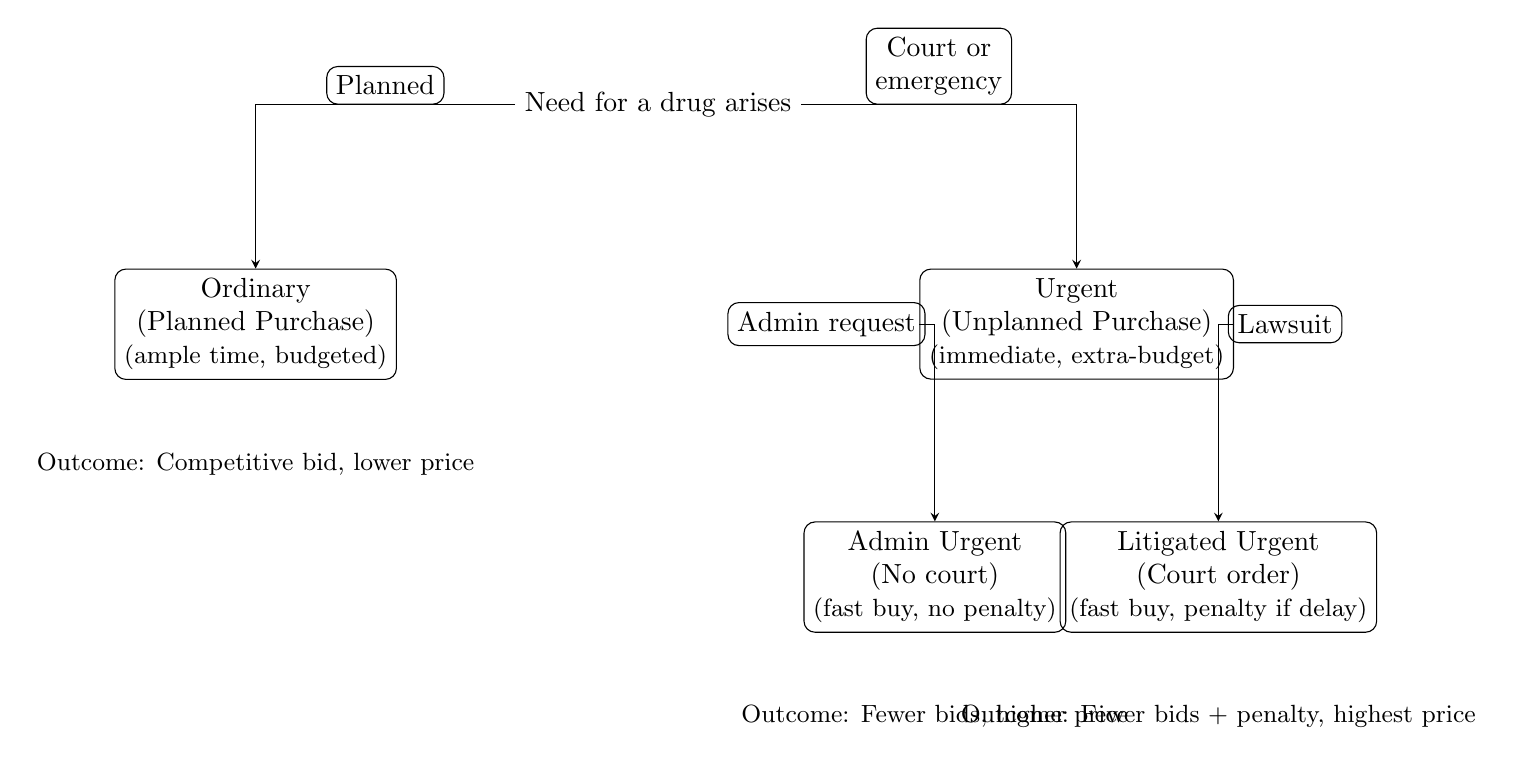
\begin{tikzpicture}[->, >=stealth, node distance=2.5cm, every node/.style={rectangle, draw, rounded corners, align=center}]
    \node (start) [draw=none, align=center] {Need for a drug arises};
    \node (ordinary) [below left=1.8cm and 1.5cm of start] {Ordinary \\ (Planned Purchase) \\ \small{(ample time, budgeted)}};
    \node (urgent) [below right=1.8cm and 1.5cm of start] {Urgent \\ (Unplanned Purchase) \\ \small{(immediate, extra-budget)}};
    \node (admin) [below=1.8cm of urgent, xshift=-1.8cm] {Admin Urgent \\ (No court) \\ \small{(fast buy, no penalty)}};
    \node (lit) [below=1.8cm of urgent, xshift=1.8cm] {Litigated Urgent \\ (Court order) \\ \small{(fast buy, penalty if delay)}};
    \draw[->] (start) -| node[above, pos=0.25]{Planned} (ordinary);
    \draw[->] (start) -| node[above, pos=0.25]{Court or\\ emergency} (urgent);
    \draw[->] (urgent) -| node[left,pos=0.2]{Admin request} (admin);
    \draw[->] (urgent) -| node[right,pos=0.2]{Lawsuit} (lit);
    \node (outO) [below=0.8cm of ordinary, draw=none] {\small Outcome: Competitive bid, lower price};
    \node (outA) [below=0.8cm of admin, draw=none] {\small Outcome: Fewer bids, higher price};
    \node (outL) [below=0.8cm of lit, draw=none] {\small Outcome: Fewer bids + penalty, highest price};
  \end{tikzpicture}
  \note{Here's a schematic of the situations we are comparing. Starting at the top, the government needs to procure a certain medicine. If everything is going according to plan (no surprises), it goes to the left branch: an ordinary planned purchase. In that branch, the government can do a normal bidding process, likely getting many suppliers to compete, which should yield a relatively low price outcome.

However, if there's a surprise need—either an administrative emergency or a lawsuit—then we go to the right branch, the urgent path. That splits into two sub-cases: If it's an administrative urgent need (no court involved), that's the left node on the bottom right. If it's a court-ordered urgent need (litigated), that's the right node on the bottom right.

In the administrative urgent case, because it’s urgent, maybe only a couple of suppliers can respond quickly or the government has to skip some steps, leading to less competition. So the price tends to be higher than in the ordinary case. In the litigated urgent case, conditions are similarly urgent but now there's also a penalty hanging if the purchase isn’t completed immediately. This pressure can cause the government to accept even higher prices (they just pay whatever to comply fast). Suppliers might also realize the government is under the gun and quote higher. So we expect the litigated urgent scenario to result in the highest price of all.}
\end{frame}

\begin{frame}{Equilibrium Predictions}
  \begin{itemize}
    \item \textbf{Ordinary vs. Urgent:} Urgent procurements lead to \textbf{higher prices} than ordinary ones.
          \begin{itemize}
            \item Urgent purchases lack the benefit of thorough planning and broad competition.
            \item Fewer suppliers or hurried negotiations $\implies$ suppliers bid less aggressively.
          \end{itemize}
    \item \textbf{Litigated vs. Non-Litigated Urgent:} Litigated urgent purchases have even \textbf{higher prices} than administrative urgent ones.
          \begin{itemize}
            \item The penalty threat (\(\gamma\)) in litigated cases acts as a \textit{markup} factor – the buyer is willing to pay more to avoid sanctions, and suppliers anticipate this.
            \item Result: \(\text{Price}_{\text{Litigated}} > \text{Price}_{\text{Admin}} > \text{Price}_{\text{Ordinary}}\).
          \end{itemize}
    \item \textbf{Competitive effect:} In ordinary tenders, many bidders drive price $\approx c$ (cost). In urgent tenders, effectively fewer bidders, price above $c$; with a penalty, price is higher still.
  \end{itemize}
  \note{Our model yields clear predictions. First, comparing an urgent procurement to an ordinary one: the urgent situation results in a higher winning price. Intuitively, when you can't plan and have to buy right away, you might not get as many bidders or you have to rush the process, so you lose some bargaining power. It's like needing to buy something last-minute; you pay a premium.

Second, if we compare a litigated urgent purchase to an administrative urgent purchase: the litigated one is predicted to be even more expensive. The reason is that the penalty threat in the litigated case means the government is extremely keen to finalize the purchase immediately, even at a bad price, because otherwise they get fined or worse. Suppliers can recognize that the government is desperate. So the presence of that penalty effectively inflates the price further. In other words, being ``under the gun'' adds an extra markup.

So in summary, we expect an ordering of prices: the lowest in ordinary procurement, higher in urgent, and highest in court-mandated urgent situations. Another way to see it is through competition: ordinarily, high competition drives the price close to the suppliers' cost. Urgency limits competition, raising prices above cost. And the penalty in litigated cases distorts things further, raising prices most of all.}
\end{frame}

\begin{frame}{Welfare Implications}
  \begin{itemize}
    \item Judicial interventions (health litigation) improve access for individual patients, but at a \textbf{social cost}:
          \begin{itemize}
            \item Government pays more per unit, meaning \textbf{budget resources are used less efficiently}.
            \item Fewer resources remain for other patients or treatments (opportunity cost).
          \end{itemize}
    \item Overall, urgent and especially litigated purchases generate \textbf{passive waste}: no one is corruptly gaining, but extra money is spent for the same good.
    \item Potential trade-off: \textit{Equity vs. efficiency} – courts enforce equity (everyone gets needed care), while the cost is spread as efficiency loss in public spending.
  \end{itemize}
  \note{What do these higher prices mean for welfare? On one hand, these court orders can save lives or greatly benefit the individuals who get their medication. That's a plus in terms of equity and individual welfare. On the other hand, the government is paying more than it ideally would. That means that for a given budget, they can afford fewer medicines overall. Money that could have been used to treat other patients or fund other health programs is instead absorbed by these expensive purchases.

Importantly, this isn't about corruption or anyone lining their pockets (which would be active waste). It's what economists call passive waste: an inefficiency in execution that causes overspending. So the welfare cost here is that the public gets less bang for its buck in healthcare.

In a broader sense, there's a policy trade-off: The judiciary is prioritizing the individual's right to health, which is very important, but the unintended consequence is a reduction in efficiency of public health spending. That tension suggests maybe we need better coordination so that we don't have to sacrifice so much efficiency to achieve equity.}
\end{frame}

\begin{frame}{Testable Hypotheses}
  From the theory, we derive two main hypotheses for the empirical analysis:
  \begin{enumerate}
    \item \textbf{Enforcement Cost Hypothesis:} \emph{Public purchases triggered by litigation or urgent administrative requests have significantly higher prices than planned purchases.}
    \item \textbf{Under-the-Gun Hypothesis:} \emph{Among urgent purchases, those under court order (litigated) are more expensive than those due to administrative urgency, due to the added pressure of potential sanctions.}
  \end{enumerate}
  \note{Now we turn these theoretical insights into concrete hypotheses that we can test with data. 

First, the enforcement cost hypothesis: if we look at purchases that were made urgently (because either a lawsuit or some urgent demand forced it) and compare their prices to similar purchases that were done in the normal planned way, we expect the urgent ones to be a lot more expensive on average.

Second, the under-the-gun hypothesis: if we focus only on urgent purchases and compare those that happened because of a court order versus those that were just administrative emergencies, the ones with a court order should on average cost more, reflecting that extra push from the judicial side.

These are precisely the effects we will measure in the data.}
\end{frame}

\section{Data and Empirical Strategy}

\begin{frame}{Data: Sources and Construction}
  \begin{itemize}
    \item \textbf{Procurement Data:} Detailed bidding records from S\~ao Paulo state's e-procurement system (BEC), covering purchases of medicines and health supplies.
          \begin{itemize}
            \item Contains tender characteristics, winning bids/prices, quantities, etc. (2009--2019).
          \end{itemize}
    \item \textbf{Health Litigation Data:} Database of individual lawsuits demanding health products in S\~ao Paulo state courts (2008--2017).
          \begin{itemize}
            \item Includes injunction dates, items requested.
          \end{itemize}
    \item \textbf{Administrative Urgent Requests:} Internal records (SES/SP) of urgent purchase requests not driven by lawsuits.
    \item We \textbf{merge} these data to identify for each tender whether it was:
          \begin{itemize}
            \item an ordinary planned purchase, 
            \item an urgent purchase due to an administrative request, or 
            \item an urgent purchase due to a lawsuit.
          \end{itemize}
  \end{itemize}
  \note{Our empirical analysis uses three main sources of data. First, we have data on public procurement from S\~ao Paulo state. This is basically the universe of purchases for health-related goods—like medications, medical equipment, etc.—made through their electronic bidding platform from 2009 to 2019. This data tells us how each tender was conducted, how much was paid, what quantities, etc.

Second, we have data on the lawsuits themselves: every lawsuit in the state courts where someone requested a free health product from 2008 to 2017. From this we know when a judge ordered the government to provide a certain drug, for example.

Third, we have data on urgent requests within the health administration. These are cases where, say, a hospital or clinic said "we're out of stock of X, we need to buy it immediately" (without a court order).

We combine these data sets. Essentially, we label each purchase in the procurement data as either a regular planned purchase, an urgent purchase triggered by an administrative need, or an urgent purchase triggered by a lawsuit. This way, we can compare across these categories in the analysis.}
\end{frame}

\begin{frame}{Data: Sample and Descriptive Stats}
  \begin{itemize}
    \item \textbf{Sample:} Public tenders for medicines and medical supplies in S\~ao Paulo state. We focus on comparable items that appear in both ordinary and urgent contexts.
    \item \textbf{Size:} Thousands of purchase records; hundreds of distinct items (pharmaceuticals).
    \item \textbf{Identification of urgency:}
          \begin{itemize}
            \item ~5--10\% of purchases are marked as urgent (either admin or litigated).
            \item Among urgent purchases, a fraction are linked to litigation (court orders); others to administrative needs.
          \end{itemize}
    \item \textbf{Baseline differences:} Urgent tenders tend to be for smaller quantities and often single-supplier bids, whereas ordinary tenders often bundle larger quantities and attract multiple bidders.
    \item Price variation of interest: We observe how the winning price for the same drug differs when bought under different conditions.
  \end{itemize}
  \note{Let me outline our analytical sample and some basic patterns. We have data on thousands of purchase instances for drugs and health supplies. Many different drug types are included, from common ones to some rarer ones. Only a minority of these purchases are urgent in nature—somewhere around 5 to 10 percent, depending on definitions. And of those urgent cases, some are because of lawsuits and some are just internal emergencies.

Even before doing any heavy analysis, we see differences: urgent purchases are usually much smaller in volume (like buying 100 doses urgently versus a normal tender for 10000 doses for the year). Urgent cases might also involve only one offer (for example, the government might call one supplier to get a quick quote) whereas ordinary cases have time to get many bids. 

So there are some inherent differences. Our strategy in analysis will account for that by comparing the same item under different scenarios, etc. But it’s clear that when the government buys under duress, it's a different process than when it buys in a planned way. The key outcome we'll focus on is the price paid. We want to see how that price changes for the same product when it's an urgent buy versus a planned buy, and further if it's a court-forced buy versus just an urgent buy.}
\end{frame}

\begin{frame}{Empirical Strategy: Enforcement Cost}
  \textbf{Idea:} Treat urgent, unplanned purchases as a ``treatment'' and compare against planned purchases.
  \medskip
  \begin{itemize}
    \item Compare outcomes (mainly price paid) for the same item when procured under normal conditions vs. under urgent mandate.
    \item Use a regression framework with item fixed effects and other controls:
          $$Price_{ijt} = \alpha + \beta \cdot Urgent_{ijt} + \lambda_{i} + \delta_{t} + X_{ijt} + \varepsilon_{ijt},$$
          where $Urgent_{ijt}=1$ if purchase $j$ of item $i$ at time $t$ was due to litigation/admin urgency.
    \item $\beta$ captures the average price difference for urgent vs. ordinary purchases (the enforcement cost).
    \item Identification: Assume that, conditional on product and time, whether a purchase is urgent (unplanned) is exogenous to factors affecting price beyond the urgency itself. (i.e. the government didn't plan it because it couldn't, not because it expected a higher price.)
    \item Check robustness with various specifications (adding controls for quantity, supplier, etc.).
  \end{itemize}
  \note{Our first empirical test looks at the enforcement cost of having to buy urgently (whether due to a lawsuit or an administrative need). We essentially compare the price of the same drug when it's bought in a regular planned tender versus when it's bought urgently because of some mandate.

Concretely, we run regressions where the dependent variable is the price paid for a drug in a given purchase. We include fixed effects for the drug itself (so we're comparing within the same drug) and possibly time fixed effects or other controls. The key independent variable is an indicator for whether that purchase was urgent (meaning it was triggered by either a lawsuit or an urgent request).

The coefficient $\beta$ on that urgent indicator tells us how much more (in percentage terms, if we log price, for example) the government paid when it had to buy urgently versus normally. The identifying assumption here is that within a given drug and time period, the urgent vs. non-urgent status is not picking up something else like quality differences—basically, the urgency is imposed by external circumstances (like someone sued or there was a stockout) not because the government only buys expensive versions of the drug urgently. We'll also add controls like quantity or number of bidders to see if that mediates the effect.

We'll test the robustness by trying different models, but the main expectation is that $\beta$ will be significantly positive, indicating a higher price for urgent buys.}
\end{frame}

\begin{frame}{Empirical Strategy: ``Under the Gun'' Effect}
  \textbf{Idea:} Within urgent purchases, isolate the effect of being court-mandated (with sanctions threat) vs. merely urgent.
  \medskip
  \begin{itemize}
    \item Restrict sample to \textbf{urgent purchases only}. Compare those with a lawsuit injunction to those without.
    \item Regression approach:
          $$Price_{ijt} = \gamma + \theta \cdot Litigated_{ijt} + \lambda_{i} + \delta_{t} + X'_{ijt} + \mu_{ijt},$$
          where $Litigated_{ijt}=1$ if urgent purchase $j$ of item $i$ was due to a court order.
    \item $\theta$ captures the additional price premium in litigated (court-ordered) tenders relative to administrative urgent tenders.
    \item Both groups face urgent timing, so difference $\theta$ isolates the effect of the legal pressure (penalty threat).
    \item Identification: Assuming that conditional on urgency, the reason (court vs admin) is not systematically correlated with unobservable cost factors (we control for item, time, etc.). Essentially, a given drug might sometimes be urgently needed due to a lawsuit and other times due to administrative issues—any systematic price difference should be due to the court's involvement.
  \end{itemize}
  \note{The second part of our strategy focuses only on urgent purchases. We want to see if having a court order (with its potential penalties) makes a difference, compared to an urgent situation that didn't involve the courts. 

So for this, we take all the urgent cases and mark whether each was litigated or not. Then we run a similar regression where the key variable is an indicator for litigated (versus administratively driven) urgency. We still include product fixed effects, etc., so effectively we're comparing the price of the same drug under two types of urgency.

The coefficient $\theta$ will tell us how much extra cost is associated with the litigated scenario. Since both types are urgent, they both lack planning and have short time frames; the big conceptual difference is the judicial pressure.

We have to assume that within a given drug, whether an urgent purchase came from a lawsuit or an administrative need is somewhat random or at least not directly tied to the price except through the mechanism we propose. It might be a strong assumption, but we try to justify that a drug that can be demanded by a patient could also be urgently needed administratively in another instance, so we do see both for some products. With controls and fixed effects, we aim to isolate that pure ``under the gun'' effect.}
\end{frame}

\section{Empirical Results}

\begin{frame}{Enforcement Cost: Urgent vs. Ordinary Purchases}
  \centering
  \includegraphics[width=0.8\textwidth]{figure4.png}
  \note{This figure illustrates the first key result: the price impact of urgent purchases compared to ordinary ones. On the screen, we see a comparison (for example, this could be a bar chart or coefficient plot) that shows how much higher the prices are when purchases are urgent.

In our analysis, we find a very large effect. Urgent purchases are on the order of 60\% to 70\% more expensive than the same items when bought through the normal, planned process. This figure visualizes that gap.

What this means concretely is if a drug normally would cost, say, \$100 per unit in a regular tender, it might cost around \$160 or \$170 per unit when the government has to buy it in a rush due to litigation or an emergency. The difference is huge, and it's a measure of the efficiency loss or enforcement cost caused by these urgent procurement scenarios.

The result shown here is statistically significant and holds consistently across various ways we slice the data or add controls.}
\end{frame}

\begin{frame}{Robustness: Across Specifications}
  \centering
  \includegraphics[width=0.8\textwidth]{figure5.png}
  \note{This figure provides a robustness check for the enforcement cost result. It likely shows the estimated price difference between urgent and ordinary purchases across multiple model specifications or subsets. 

As we can see, regardless of how we estimate it—whether we control for additional factors like quantity or supplier fixed effects, or use different subsets of data—the urgent purchases consistently come out much more expensive than ordinary ones. The estimates cluster around that 60-70\% increase range.

For instance, one model might include product and year fixed effects, another might add controls for how many bidders participated, another might separate branded drugs versus generics. In all cases, the price in urgent tenders is significantly higher. 

This builds confidence that our finding isn’t a fluke of one particular method; it’s robust. Urgency itself, not some other hidden variable, is driving up the cost. In summary, no matter how you cut it, the enforcement cost is real and substantial.}
\end{frame}

\begin{frame}{Why Are Urgent Purchases Costlier?}
  \begin{itemize}
    \item \textbf{Lack of Planning:} The government cannot consolidate demand or schedule purchases optimally.
    \item \textbf{Smaller Quantities:} Urgent orders often for a single patient or immediate need $\implies$ lose bulk discounts.
    \item \textbf{Shorter Timelines:} Less time for suppliers to prepare bids or for the government to seek alternatives $\implies$ reduced competition.
    \item \textbf{Procedural Flexibility:} Urgent cases may use simplified or non-competitive procurement methods (e.g., direct contracting due to emergency rules).
    \item \textbf{Supplier Leverage:} Suppliers know the buyer is desperate (especially if it's public knowledge it's an injunction) and may charge premium prices.
  \end{itemize}
  \note{We found that urgent purchases are much more expensive, but let's discuss why that is the case.

Firstly, when a purchase isn't planned, the government can't do things like combine orders or carefully time the market. They lose the efficiencies of planning.

Secondly, these urgent buys are usually small. Instead of buying a year’s supply for the whole state, you might be buying one patient's dose or a one-month supply. Buying in small batches usually means paying a higher unit price; you don't get volume discounts.

Third, the timeline is extremely short. With maybe just a few days to arrange the purchase, there's no chance to invite many bidders or negotiate much. Some potential suppliers might not even hear about the tender in time. This naturally leads to less competition.

Fourth, because of the urgency, procurement officials might be allowed to bypass normal competitive bidding rules—like they might be allowed to do a sole-source contract if it's an emergency. While that speeds things up, it often means you don't get the lowest price.

And finally, suppliers are aware that when the government comes calling last-minute for a drug, it's likely an emergency. Especially if they know it was a court order (sometimes these things are public or known in the industry), they realize the government has no choice. That increases the bargaining power of the supplier, who can then quote a higher price. 

All these factors contribute to why we see such a big price gap in urgent purchases. Essentially, the government is paying for the luxury of immediacy and certainty of supply.}
\end{frame}

\begin{frame}{Under-the-Gun Effect: Litigated vs. Admin Urgent}
  \centering
  \includegraphics[width=0.75\textwidth]{figure6.png}
  \note{Now we turn to the second question: among those urgent purchases, does it make a difference if the urgency is due to a court order? This figure focuses only on urgent cases and compares prices between litigated and non-litigated ones.

The analysis reveals a clear under-the-gun effect. When a purchase is urgent \emph{and} court-ordered, it tends to be even more expensive than an urgent purchase triggered by administrative reasons. In our estimates, litigated urgent purchases are roughly 9-10\% more expensive than otherwise identical urgent purchases without a court order.

This figure illustrates that premium. For example, if an administratively urgent purchase might cost \$170 (relative to \$100 normal), a litigated urgent purchase of the same item might cost around \$185 or so. That extra difference is attributable to the presence of the judicial pressure.

Statistically, this effect is smaller than the overall urgent vs. non-urgent gap, which makes sense—both cases are already urgent, so they share a lot of cost-increasing factors. But this additional bump of roughly 9\% is consistent and significant. It's the cost of being ``under the gun'' of the judiciary.}
\end{frame}

\begin{frame}{Robustness: Isolating the Penalty Effect}
  \centering
  \includegraphics[width=0.75\textwidth]{figure7.png}
  \note{This figure provides some robustness and nuance for the under-the-gun effect. It likely shows the litigated vs. admin price difference across different specifications or subgroups, similar to what we did before.

The results consistently show a positive premium for litigated purchases, on the order of roughly 9\%. Some bars or points might correspond to different ways of controlling for factors. For instance, controlling for the number of bidders, or focusing on drugs that had multiple urgent purchases of both types, etc. The consistency of the positive difference gives us confidence that the court involvement itself is adding cost.

One interesting thing is that while the percentage may seem smaller compared to the 60\% urgent effect, this 9\% is on top of an already high price. And remember, this is basically an inefficiency caused purely by the legal sanction environment. We see that even when urgency and product are the same, just the threat of punishment to the buyer yields a noticeable price increase.

Thus, even within urgent scenarios, the mechanism of enforcement (judicial vs. administrative) matters.}
\end{frame}

\begin{frame}{Interpreting the Under-the-Gun Effect}
  \begin{itemize}
    \item When under a court injunction, officials behave differently:
          \begin{itemize}
            \item They are \textbf{less price-sensitive} -- priority is to fulfill the order immediately to avoid fines or contempt.
            \item Procurement officers may choose faster but costlier procurement methods (e.g., single-source) to ensure compliance.
          \end{itemize}
    \item Suppliers exploit the situation:
          \begin{itemize}
            \item Recognize the government \textit{must} buy no matter the price $\implies$ quote higher offers.
            \item No threat of the buyer walking away or delaying (since delay is not an option under court order).
          \end{itemize}
    \item \textbf{Net effect:} An extra $\sim$9\% price premium on top of usual urgency costs, purely due to legal pressure.
    \item This is effectively a \textbf{penalty-driven markup} in the market, representing an additional welfare loss imposed by judicial enforcement.
  \end{itemize}
  \note{So why does having a court order add about 9\% more to the cost? It comes down to behavior under pressure.

From the government's side, once a judge is involved, the procurement officials' top priority is to satisfy the court as quickly as possible. They become less concerned about getting the best price deal. For example, they might skip trying to negotiate or skip waiting for a possibly cheaper supplier if that could risk missing the judge's deadline. They might do a direct purchase from a known supplier who can deliver immediately, even if it's more expensive, just to ensure they obey the order.

From the suppliers' side, if they know the government is under legal pressure and basically cannot say no, that gives the suppliers more power. The government isn't going to cancel the purchase even if the price is high, because they can't fail to buy the item. So suppliers might raise their prices or not offer any discount they might have offered otherwise. They know the buyer is essentially captive.

So combining those, the legal pressure translates into an extra price premium of roughly 9\%. This is like a special kind of markup that only appears because of the enforcement mechanism. In terms of welfare, it's an additional cost that doesn't benefit the supplier much either beyond a one-time gain, and it's money straight out of the public coffer due to how the enforcement is structured.}
\end{frame}

\begin{frame}{Summary of Key Results}
  \begin{table}[ht]
    \centering
    \begin{tabular}{lcc}
      \toprule
      & \textbf{Price Increase} & \textbf{Other Effects} \\
      \midrule
      \textbf{Urgent vs. Ordinary} & +65\% (approx.) & - Planning, - Competition, - Quantity \\
      \textbf{Litigated vs. Admin (urgent)} & +9\% (approx.) & + Legal pressure, + Risk to officials \\
      \bottomrule
    \end{tabular}
  \end{table}
  \vspace{1em}
  \begin{itemize}
    \item Urgency imposes a large efficiency cost on procurement (prices much higher).
    \item Judicial involvement adds a noticeable extra cost on top of urgency.
    \item Both findings align with model predictions: $Price_L > Price_A > Price_O$.
  \end{itemize}
  \note{Let's recap the core findings in a succinct way. We have two big comparisons:

First, urgent vs ordinary purchases. We find about a 65\% increase in price on average when a purchase is urgent. It's a huge difference. This is accompanied by things like less planning, reduced competition, and smaller purchase sizes in those urgent scenarios, all of which contribute to that higher price.

Second, within urgent purchases, the presence of a litigation (the under-the-gun scenario) leads to roughly an additional 9\% increase in price compared to an administrative urgent purchase. This difference is specifically due to the legal pressure on officials, which isn't present in the admin case.

These results confirm our theoretical predictions that litigated urgent purchases would be the most costly, followed by administrative urgent, and then ordinary being the least.

In short: there's a big efficiency penalty to urgent, unplanned procurement, and an extra penalty when that urgency is enforced by courts.}
\end{frame}

\section{Conclusion and Discussion}

\begin{frame}{Conclusion}
  \begin{itemize}
    \item \textbf{Enforcement costs are substantial:} Judicial (and urgent administrative) interventions in health procurement lead to significantly higher costs. The government spends much more per unit when forced into urgent action.
    \item \textbf{Mechanism confirmed:} Urgent purchases suffer from low competition and haste, and court-ordered cases further suffer from penalty-driven distortions. 
    \item We quantify these effects: about 65\% price increase due to urgency, and an additional ~9\% due to being under judicial “gun”.
    \item \textbf{Implication:} While litigation can save individual lives, it induces inefficiencies that can undermine the broader healthcare budget.
  \end{itemize}
  \note{In conclusion, our study shows that there are indeed bitter pills in the form of enforcement costs. When courts or emergencies compel the government to make an unplanned purchase of medication, it ends up paying a lot more—on the order of tens of percent more—than it would under normal circumstances. This is a significant inefficiency.

We delved into why that is the case and found evidence supporting the idea that it’s driven by the nature of urgent procurement—less competition, less planning—and in the case of litigated ones, the pressure of penalties.

Quantitatively, these are not trivial numbers: roughly a two-thirds increase in price for urgent situations, and even within those, nearly a ten percent additional jump if it’s a court-mandated purchase.

This suggests that while the judiciary’s intentions are to fulfill rights and help individuals, these interventions are actually quite costly for the public budget. In other words, there's a trade-off: those individual health needs are being met, but at a cost of general efficiency that could have consequences for how many resources remain to help others.

Now, knowing these numbers, we can discuss what might be done about it.}
\end{frame}

\begin{frame}{Policy Implications}
  \begin{itemize}
    \item \textbf{Better Coordination:} Develop mechanisms for courts and health authorities to coordinate. For example, a fast-track procurement channel that is pre-planned for likely litigation demands, to reduce last-minute scramble.
    \item \textbf{Information Sharing:} Judges could consult with health administrators about the cost and time implications before issuing orders, possibly allowing more reasonable deadlines or group purchasing of multiple cases.
    \item \textbf{Guidelines for Judiciary:} Encourage consideration of budgetary impact in judicial decisions. Perhaps require an assessment of whether the needed drug is already being procured or if a short delay could save costs.
    \item \textbf{Preventive Policies:} Government should try to reduce the root cause of litigation by ensuring availability of essential medicines proactively, so fewer patients feel the need to sue.
    \item Ultimately, address the equity-efficiency trade-off: aim to guarantee the right to health \emph{and} protect the public purse by mitigating the conditions that cause massive inefficiencies.
  \end{itemize}
  \note{Given these findings, what can be done to mitigate these enforcement costs? 

Firstly, better coordination between the judiciary and the executive could go a long way. If courts understood the procurement process constraints, they might tailor their orders in a way that gives just enough time for a somewhat competitive process. For instance, if they know a certain expensive drug often triggers lawsuits, the health department and courts could have an arrangement to handle it via a special procurement program rather than chaotic emergency buys.

Sharing information is crucial: maybe a judge can ask the health agency, "Can you get this drug? How long would you need without incurring huge costs?" Or the health agency can inform the courts regularly about what high-cost items are in short supply and what the plan is to get them, so the courts don't prematurely intervene.

We could also have guidelines or training for judges to make them aware of these economic impacts. The goal isn't to deny patients, but maybe to find a way to consolidate orders or avoid ordering something in an extremely short timeframe if it could be done a little more efficiently with slight adjustments.

The government on its end should also see this as a signal: if so many people are suing for a drug, maybe it should be included in the public provision plans in the first place, to preempt the need for lawsuits.

In short, bridging the gap between ensuring everyone's health needs are met and doing so in a cost-effective way is the challenge. Our findings highlight the cost side of the equation, and we hope policymakers use this evidence to improve the process and reduce waste.}
\end{frame}


\begin{frame}{Thank You}
  \centering
  \Large{Thank you!\\[1ex]Q \& A}
  \note{Thank you all for listening. I welcome any questions or comments you have about this research.}
\end{frame}

\end{document}
